\documentclass{article}
\usepackage{graphicx}
\title{Invasive Species Profile: The Burmese Python}
\author{Joshua Reed \\ Oregon State University}
\date{Fall, 2017}

\begin{document}

\maketitle

\section*{Introduction}

\paragraph{Outline}
Reproduction
The Burmese Python are R-selected, and most of the offspring die at a young age. While the Burmese Python is an apex predator, it is also preyed upon. The
Burmese Python is most vulnerable before it reaches its large size. 

Competitive Strategies


Origins to America. Hurricane Andrews caused release from a private breeding facility. See nature NPR article or Nonnatives --- Burmese Python

Distribution and Rate of Spread (Map?)
\begin{centering}
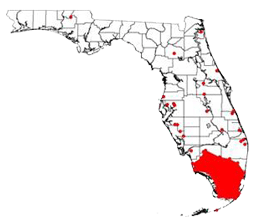
\includegraphics[scale=0.5]{Burm-Florida-range-map.png}
\end{centering}

Ecological Impacts

Economic Impacts



\section*{Body}\label{documentclasses}

\begin{description}
\item[article\label{article}]{Article is \ldots}
\item[book\label{book}]{The book class \ldots}
\item[report\label{report}]{Report gives you \ldots}
\item[letter\label{letter}]{If you want to write a letter.}
\end{description}


\section*{Conclusion}\label{conclusions}
There is no longer \LaTeX{} example which was written by~\cite{doe}.


\begin{thebibliography}{9}
\bibitem[Doe]{doe} \emph{First and last \LaTeX{} example.},
John Doe 50 B.C. 
\end{thebibliography}

\end{document}
